\section{Performance Evaluation}\label{sec:pros_perf_eval}

\todo{Closeup of final design}
\todo{Pictures of test rig}
\begin{figure}[htb]
    \centering 
    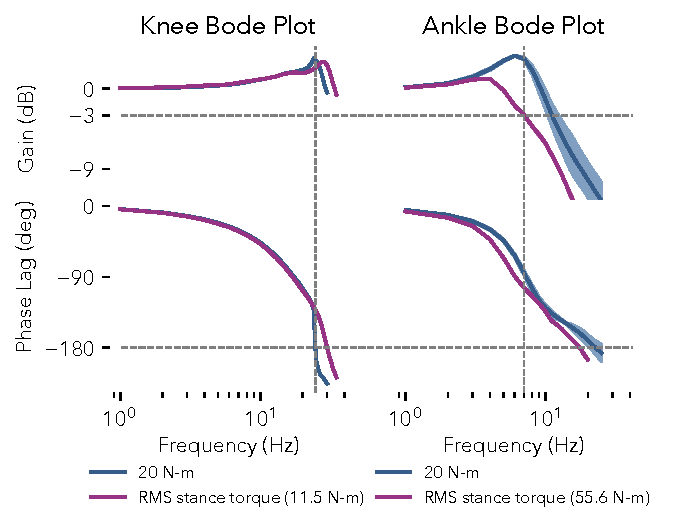
\includegraphics[width=\textwidth]{bode_plot_fixed_labels}
    \caption{Experimentally obtained bode plots of knee and ankle actuator
    torque. Knee is phase limited at \unit[24]{Hz} while the ankle is gain
    limited at \unit[7]{Hz}.}\label{fig:pros_design_bode_plots}
\end{figure}

\begin{figure}[htb]
    \centering 
    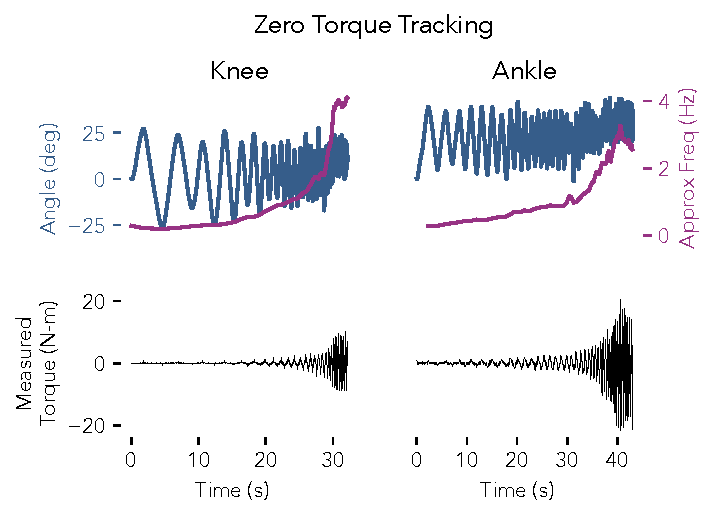
\includegraphics[width=\textwidth]{zero_torque}
    \caption{Zero torque tracking of knee and ankle joints. The prosthesis was
    fixed to a rigid mount and commanded to maintain zero net joint torque while
    the knee and ankle joints were manually oscillated (blue) by hand at
    increasingly fast rate (purple). The resulting measured torque is shown in
    the second row of axes in black.}\label{fig:pros_design_bode_plots}
\end{figure}

\todo{torque tracking during walking RMS error}
